\documentclass{article}
\usepackage{graphicx}
\usepackage{amsmath}
\usepackage{amssymb}
\usepackage{array}
\usepackage{subfigure}
\title{Estimating Markov Random Field Parameters for the model prior}
\author{Alex Kass}
\date{3/20/2011}

\begin{document}
\section{Markov Random Fields}
%
%make .pdf of image
%run to convergence
%describe MRF
%document MRF that we've defined (equations for every function)
%matrix S
%dimensions 245 x length of score
%equations for all features
%p(S) = (...)
%figure with sample input score (with labels corresponding to notation)
%figure (one typical sample from randomly generated score)

A Markov Random Field, or undirected graphical model, provides a representation of non-directional influences among nodes within a network.  Two critical properties of an MRF are conditional independence and factorization, illustrated by the following respective equations:

\begin{eqnarray*}
\Pr(\mathbf{X}) = \prod_i{\Pr(x_i \mid x_{neighbors(i)})}\\
\Pr(\mathbf{X}) = \prod_i{\Pr(x_i, x_{neighbors(i)})}
\end{eqnarray*}

The joint probability of an MRF can be seen as the product of its clique potential energy functions, where a $clique$ is a fully connected subset of nodes, and its potential function $\psi_\theta(x_\theta)$ is 
\begin{eqnarray*}
\psi_\theta(\mathbf{x}_\theta) = \exp\{-H_\theta(\mathbf{x}_\theta)\}
\end{eqnarray*}

Here, $H_\theta$ represents the energy function of a specific clique based on a single parameter $\theta$, and will vary with our MRF parameter constructions as defined in the subsequent section.  We employ the exponentials as a computational convenience, given that our potential functions always represent positive values.  This allows us to calculate the total energy by adding the energies for each of the cliques.  Incorporating $Z(\Theta) = \sum_{\mathbf{x}}\prod_{cliques_\Theta}{\psi_\Theta(\mathbf{x}_\Theta)}$ as the $partition function$, or normalizing constant, we have the joint probability over all nodes $\mathbf{X}$ and cliques $\Theta$ as:
\begin{eqnarray*}
\Pr(\mathbf{X}) = \frac{1}{Z}\prod_{cliques_\Theta}{\psi_\Theta(\mathbf{x}_\Theta)}
\end{eqnarray*}

Thus, to construct our particular MRF, we must define the various potential functions through constrcuting representations of their respective parameter energy functions.


\section{Designing a set of musical MRF parameters for the model prior}

When choosing the nature of the parameters of our Markov Random Field, we want to err on both sides of the musical generality/specificity argument.  For example, we've designed one parameter that measures whether a note stays the same or changes (denoted within the model as $\beta$).  In comparison, we designate another parameter ($\lambda$) arbiter of the likelihood of a specific note movement (e.g. moving up a whole step on a standard Western scale) and aggregate all possible note movements within an instrument's four octave range.  Another parameter involves measuring how close a specific voiced note is to the middle of an instrument's range (notated as $\alpha$, utilizing the weighted matrix M).  A final set of parameters (seen as $\varkappa$) measures the tendencies of certain harmonies to appear within a score - for example, there should be different weights on consonant intervals such as major thirds versus dissonant intervals such as a half-step or a tri-tone (6 half-steps).  On this, we truncate the four-octave range into a single one (modulo 12 to create a single, 12-note range), so as to emphasize the import of the relative fundamental scale frequencies within an interval's spectrum, rather than distinguishing between three half steps and a minor third three octaves apart.

As intimated in the first section, to calculate the joint probability of the parameter space, we multiply all clique potentials together while normalizing by a partition function $Z\left(\Theta\right)$.  By taking the $\log$ of both sides of the equation, we can ease computation by simply adding the individual parameter components together within the exponential term on the right side.  Here, we calculate the derivative of the log of the joint probability for Score $k$ with respect to the parameter space $\Theta$, where $\varkappa$ and $\lambda$ are 12x1 and 95x1 parameter vectors, respectively:

\begin{eqnarray*}
\lefteqn{\frac{\partial}{\partial\Theta}\log{\Pr\left(S_k|\Theta\right)}}  \\
&=& \log{\frac{1}{Z\left(\Theta\right)}\exp\{-\alpha\sum_v\sum_b{S_{vb}M_{vb}}- \beta\sum_v\sum_b{(S_{vb}-S_{v,b-1})^2} - \varkappa\sum_{b}{H_b} - \lambda({J})\}}
\end{eqnarray*}


Each 12x1 vector $H^b$ is an aggregate total of harmonic intervals (normalized to fall within a single octave and indexed by $int$) at a specific beat $b$.  It determines all possible pairwise interval combinations from the five notes (${5\choose2}$=10) that are on at a given time step.  $\zeta_i^b$ represents the linear index of the note that is "on" at time $b$ in instrument part $i$:

\[H_{int}^b = \sum_{i=1}^4\sum_{j=i+1}^5\mathbb{1}\left(\left|\zeta_i^b-\zeta_j^b\right|\bmod{12} = int\right)\]

As seen above, the $\lambda$ parameter (this being a 95x1 vector) is multiplied by $J$, which itself is a vector of the sums of each of the 95 interval jumps (here indexed as $int$), tabulated within each of the five instruments ($i$) throughout the duration of the score.  Thus, $\zeta_{b,i}$ holds similar information as the preceding equation:

\[J_{int} = \sum_{b=2}^{B}\sum_{i=1}^5\mathbb{1}\left(\left|\zeta_{b,i}-\zeta_{b-1,i}\right| = int\right)\]

\section{Prototype MIDI Score matrices as parameter training}

We found multiple MIDI quintet scores of different genres to incorporate into a cell array of prototypes with which to initialize our Markov Random Field prior learning process.  These range from classical brass quintets to five-part arrangements of popular tv theme songs, so that the diversity of compositional technique and harmony would provide a broader learning environment.  Each score (in the form of a binary matrix $S$) has five instrument parts, with four octaves of twelve notes each + one placeholder per part for musical rests = 245 total pitch rows (denoted as $V$).  The number of columns (denoted as $B$) varies with the length of the scores, but is generally taken to be at a resolution of one beat per sixteenth note at common time (4/4 time signature).  An example score (an extract from Handel's "Water Music") is seen in Figure 1.

\begin{figure}
\centering
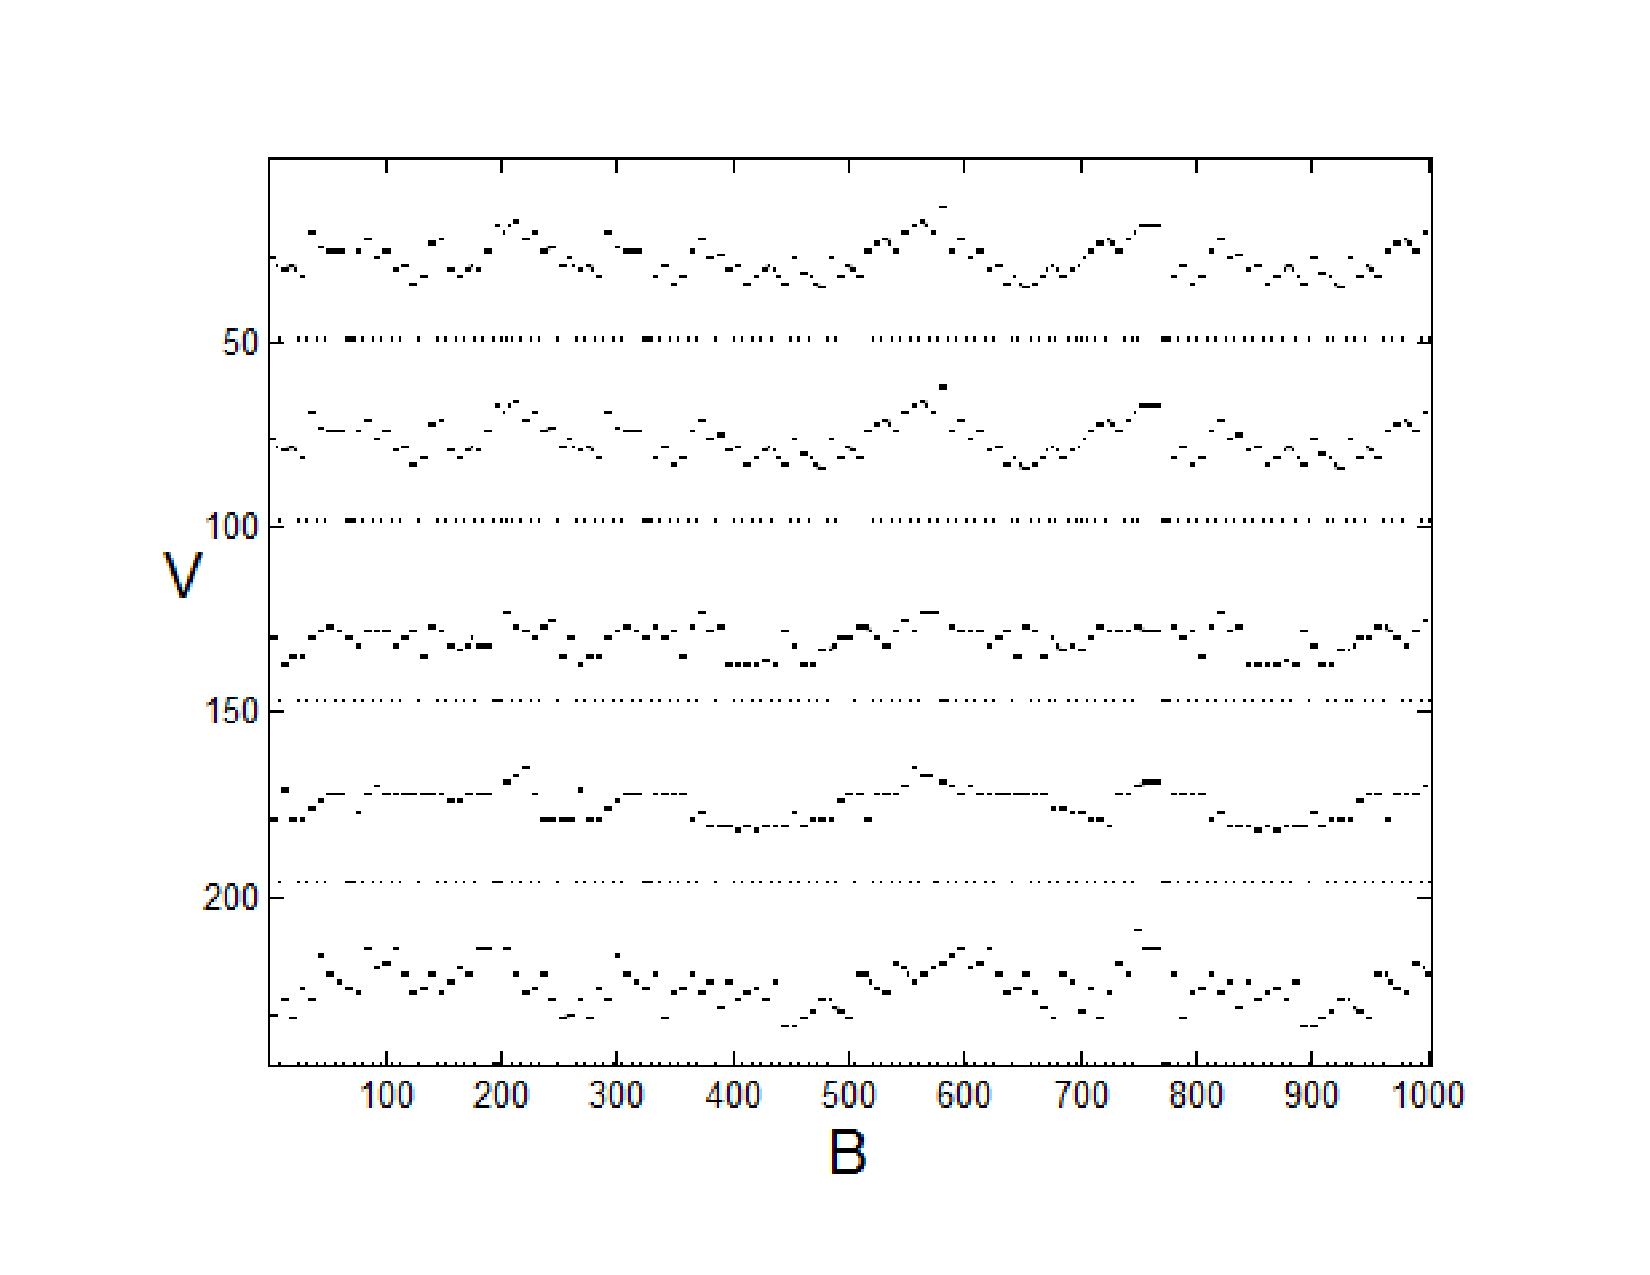
\includegraphics[width=.9\textwidth]{figures/handel(extract).pdf}
\caption{An extract of Handel's "Water Music" in $S$ format, with $V$ = individual pitches for concatenated parts, $B$ = \# of time instances throughout score.  Note the rests occuring every 49th pitch.}
\label{fig-1}
\end{figure}


\section{Estimating parameters through MCMC and Contrastive Divergence}
We employ a Metropolis-Hastings sampler to draw from the array of prototype scores, updating each of the parameters accordingly.  Further, using Contrastive Divergence, we're able to move the parameter estimates along towards convergence via gradient ascent, using the notion that the a single parameter's component of the gradient is proportional to the difference between the expectation of the log of the derivative with respect to that parameter over the original score data and that of the newly sampled score data.  Referencing the combined parameter space $\Theta$, and moving along the gradient so as to minimize the energy function of the MRF, we have the update function:

\[\Theta_{t+1} = \Theta_t + \eta\nabla_{\Theta}\]

where $\eta$ is the set of learning rates for the parameters, determined experimentally, and

\[\nabla_{\Theta} = \langle\frac{\partial\log{f(x;\Theta)}}{\partial\Theta}\rangle_{X^0} - \langle\frac{\partial\log{f(x;\Theta)}}{\partial\Theta}\rangle_{X^s}\]

Contrastive divergence allows us to approximate the gradient for the parameters by iterating only a few times through the MCMC process, which speeds up computation considerably.  In the above equation, $X^s$ represents the sth iteration of sampling the data X.

Once the parameters have been estimated to the point of convergence, we set them as the prior and proceed to subsequent signal processing.  Figure 2 shows the convergence of the $\beta$ and "major 3rd" component of the $\varkappa$ harmonic interval vector component over 40,000 iterations of sampling.  We measured convergence based on the asymptotic movement of the joint log likelihood and norm of the gradient.

\begin{figure}
\centering
\mbox{
\subfigure{
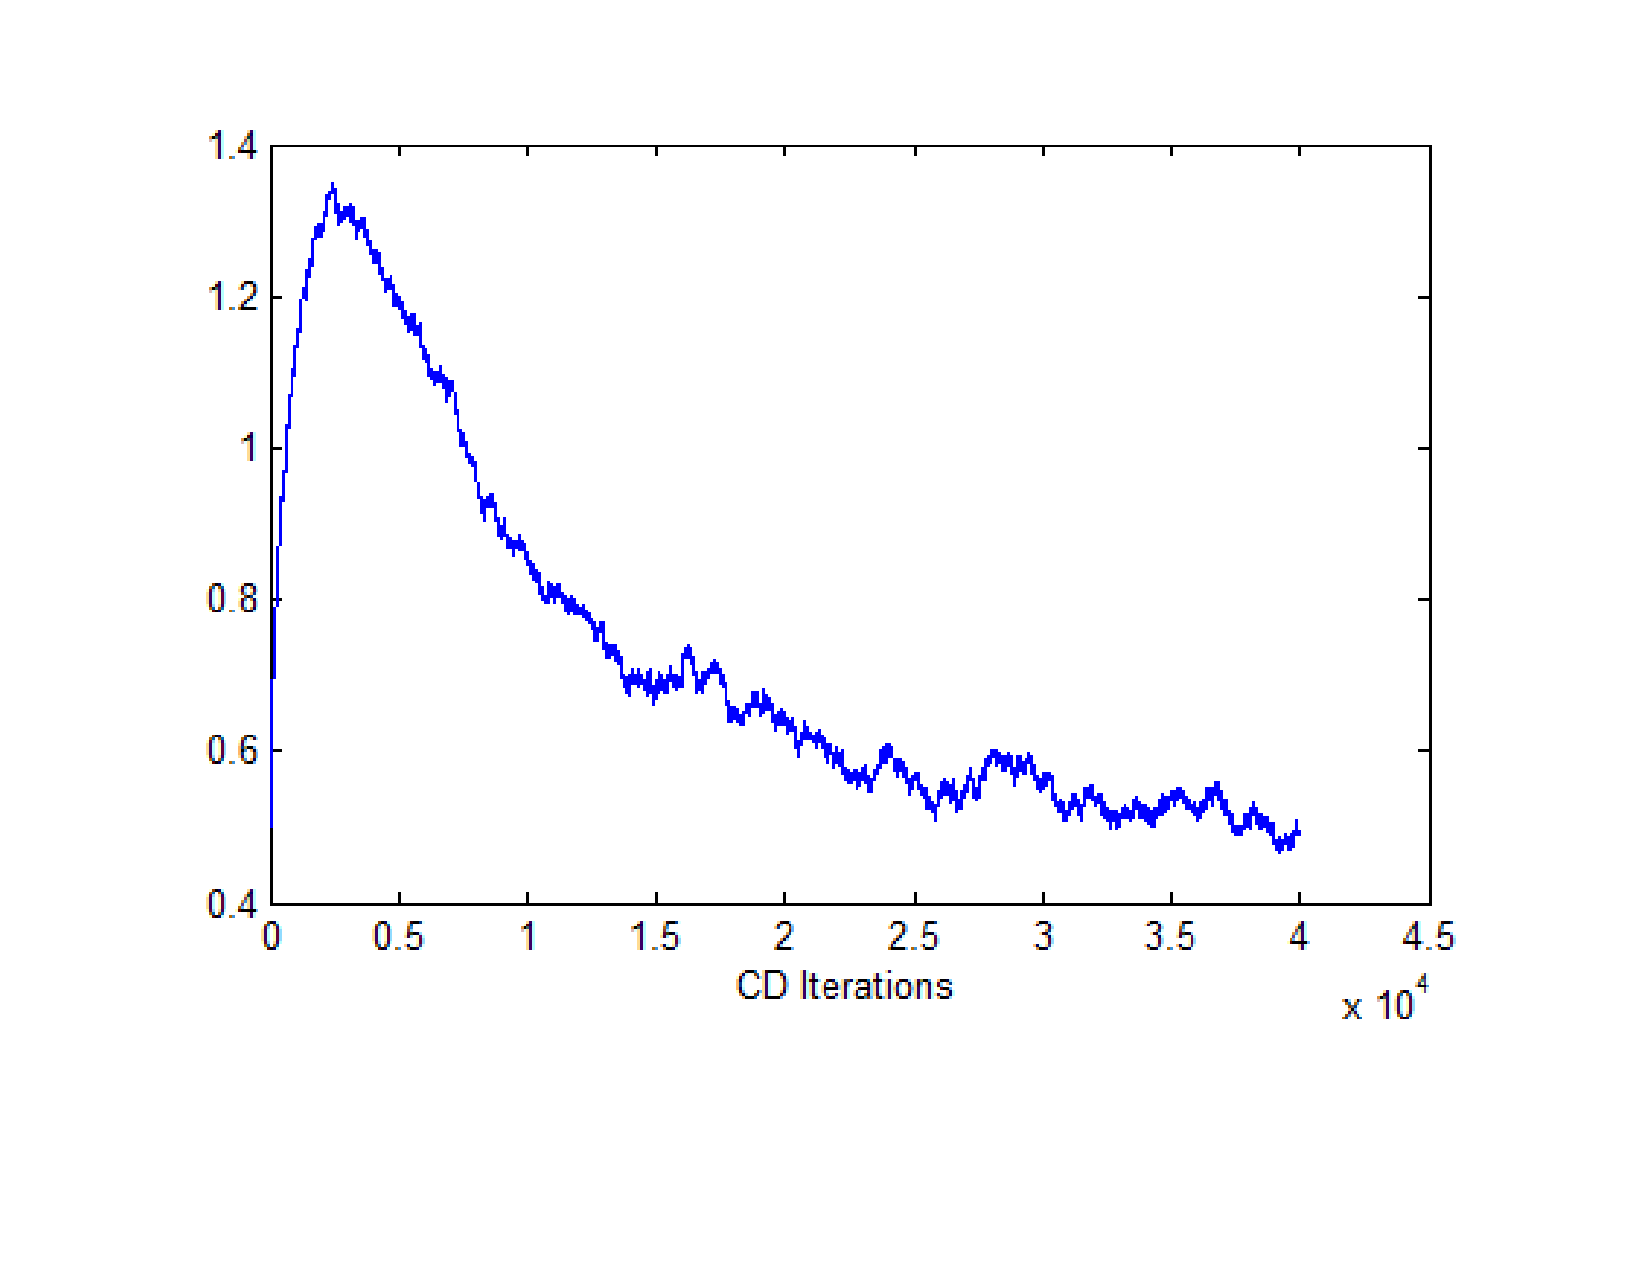
\includegraphics[width=.25\textwidth]{figures/alpha.pdf}
\label{fig-2}
}\quad
\subfigure{
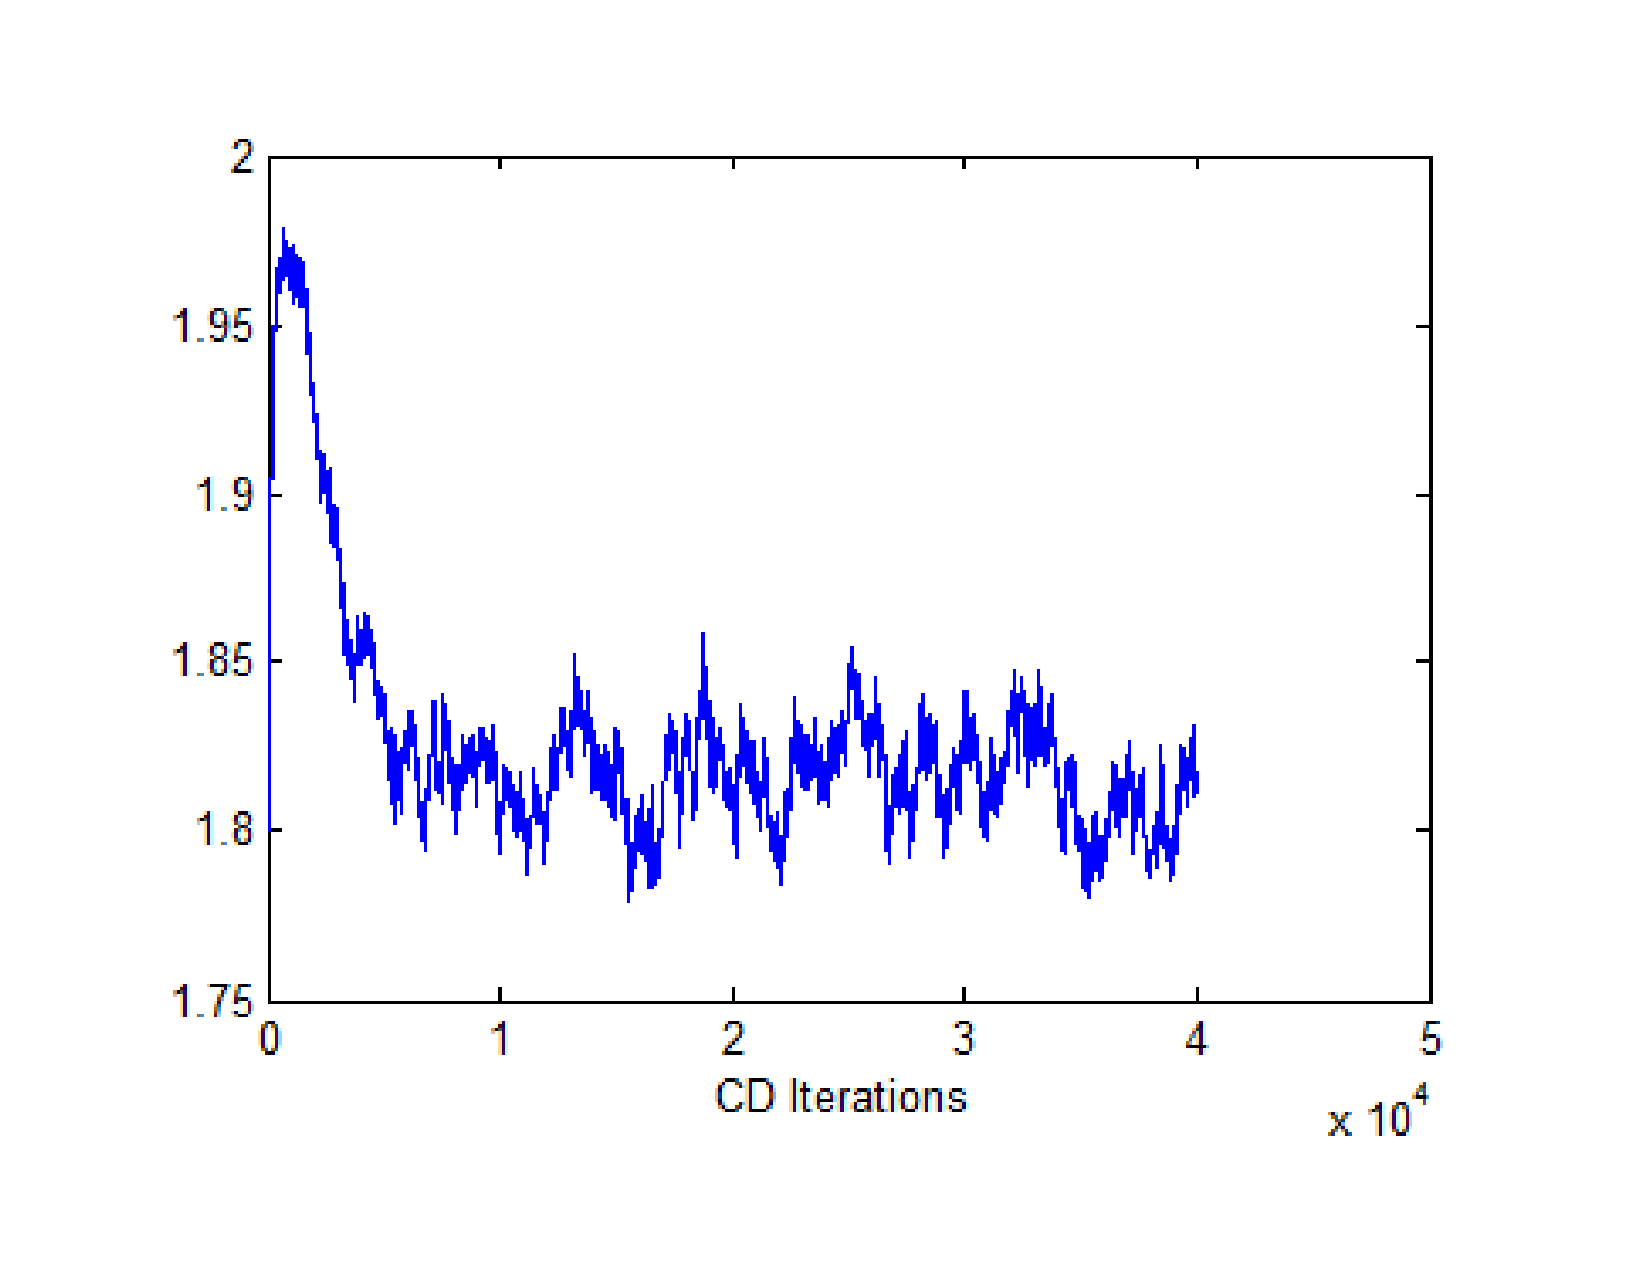
\includegraphics[width=.25\textwidth]{figures/beta.pdf}
\label{fig-3}
}\quad
\subfigure{
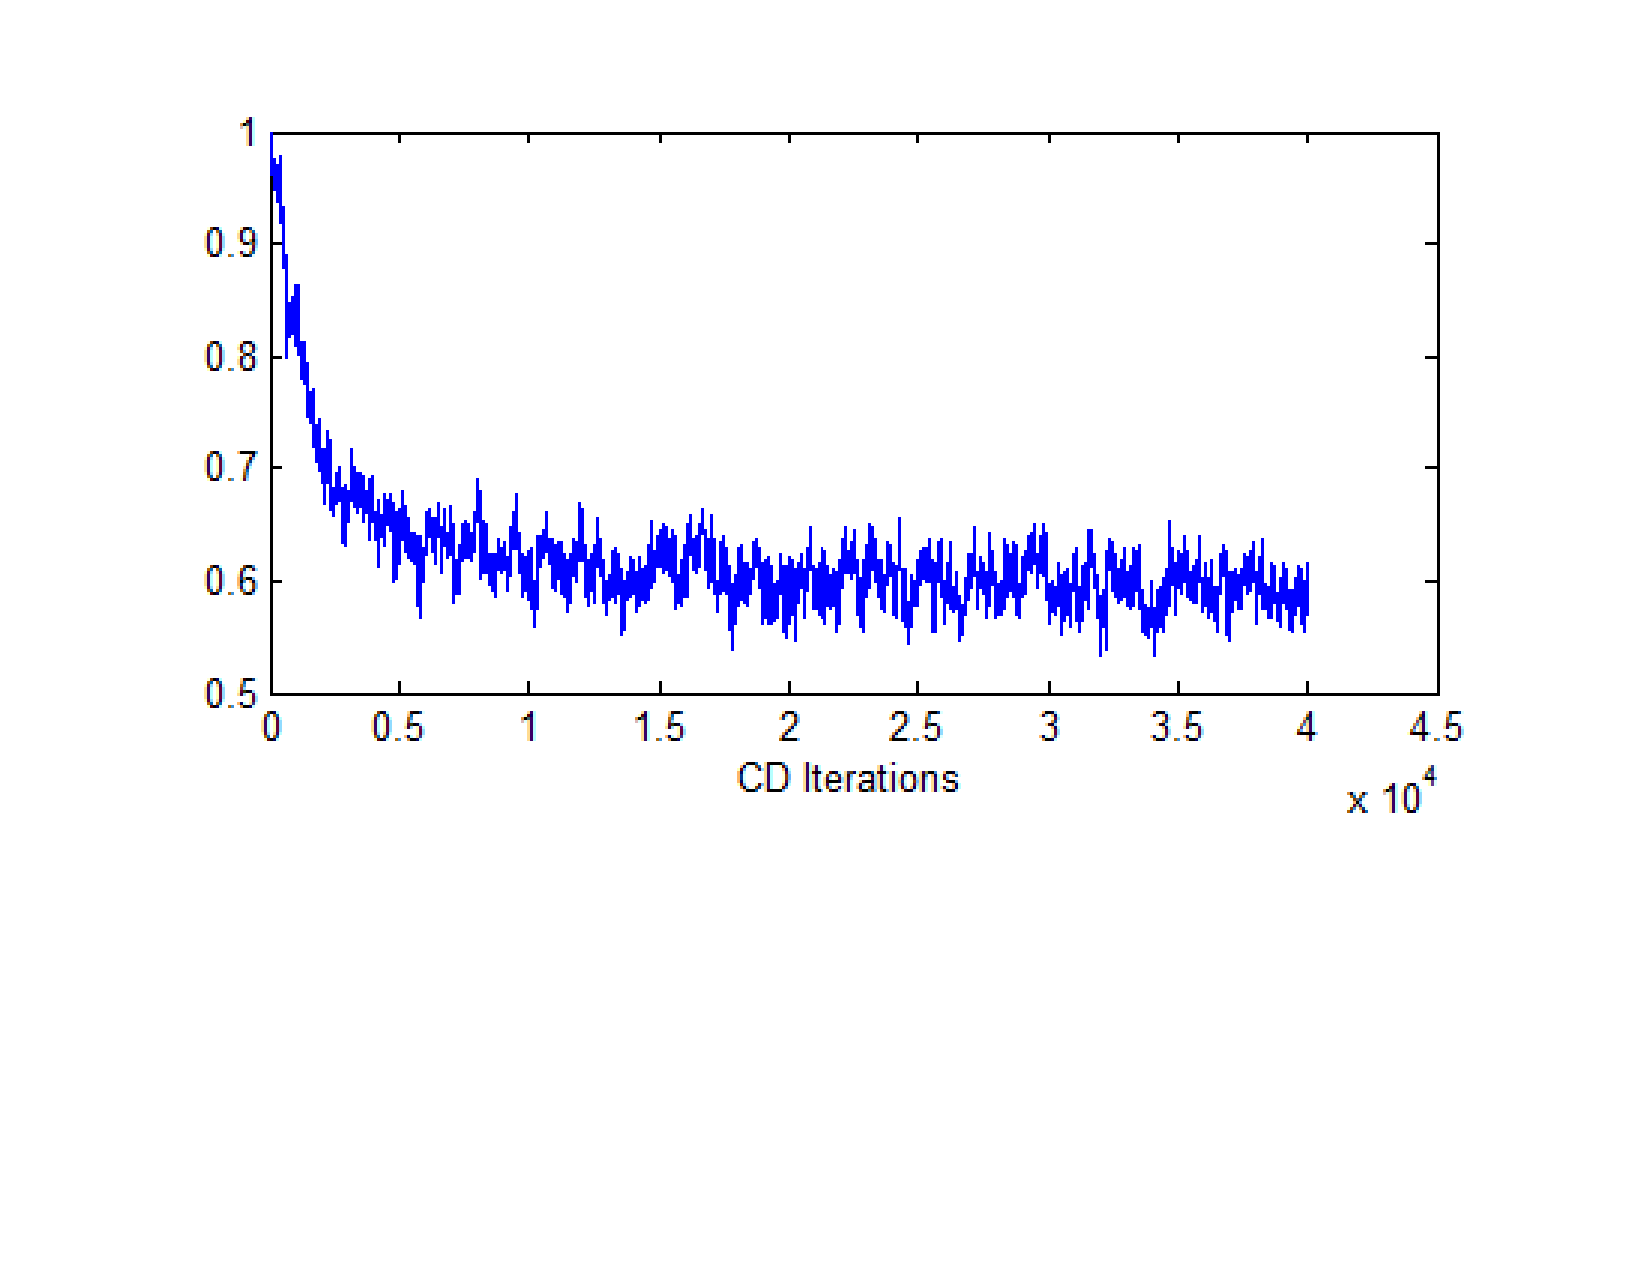
\includegraphics[width=.25\textwidth]{figures/harmony(M3).pdf}
\label{fig-4}
}\quad
\subfigure{
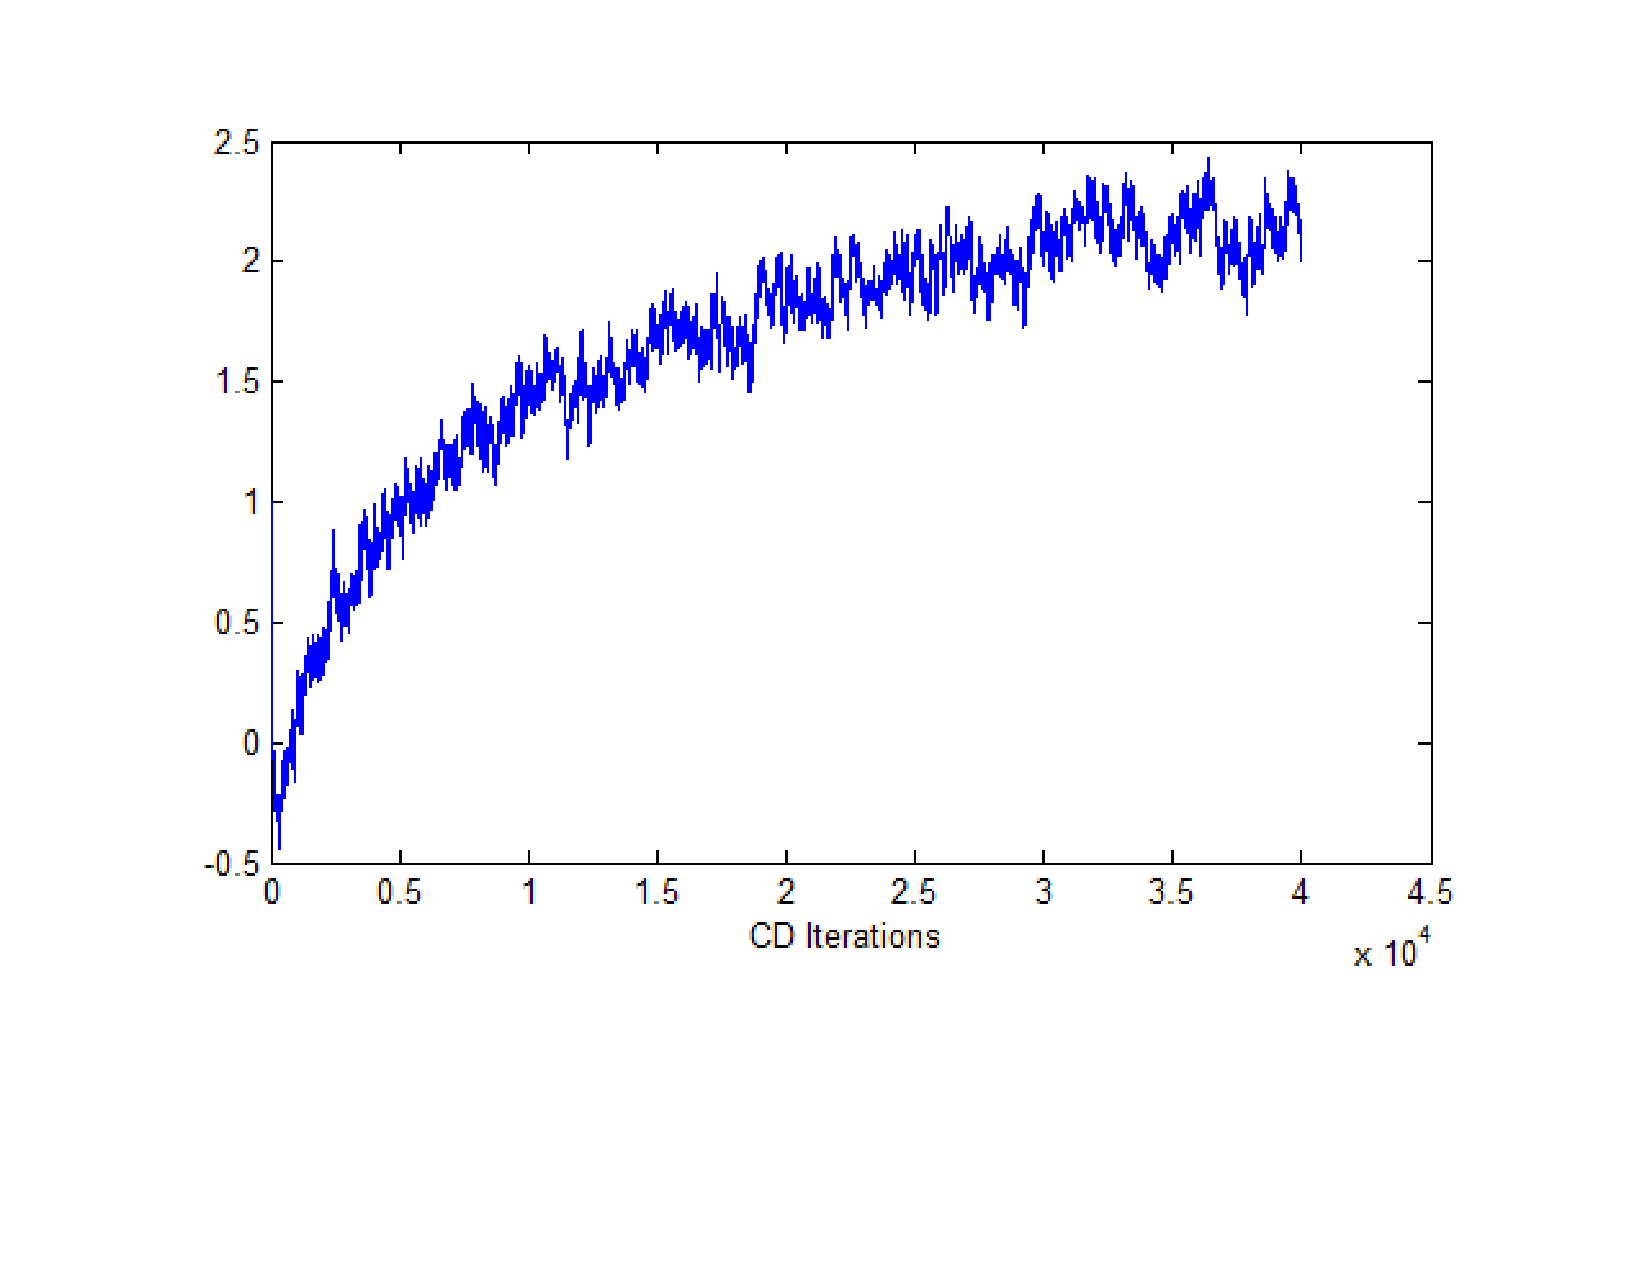
\includegraphics[width=.25\textwidth]{figures/note_movement(downhalfstep).pdf}
\label{fig-5}
}
}
\centering
\caption{Convergence of $\alpha$, $\beta$, $\varkappa$ (Major 3rd interval), and $\lambda$ (down 1/2 step) parameters over 40,000 sampler iterations using 3 Contrastive Divergence sweeps per sample.}
\label{fig-all}
\end{figure}

We can demonstrate the effect of our learned parameters by generating a random score and observing the same score after it has been sampled 1000 times using the new parameters, as seen in Figure 3.

\begin{figure}
\centering
\mbox{
\subfigure{
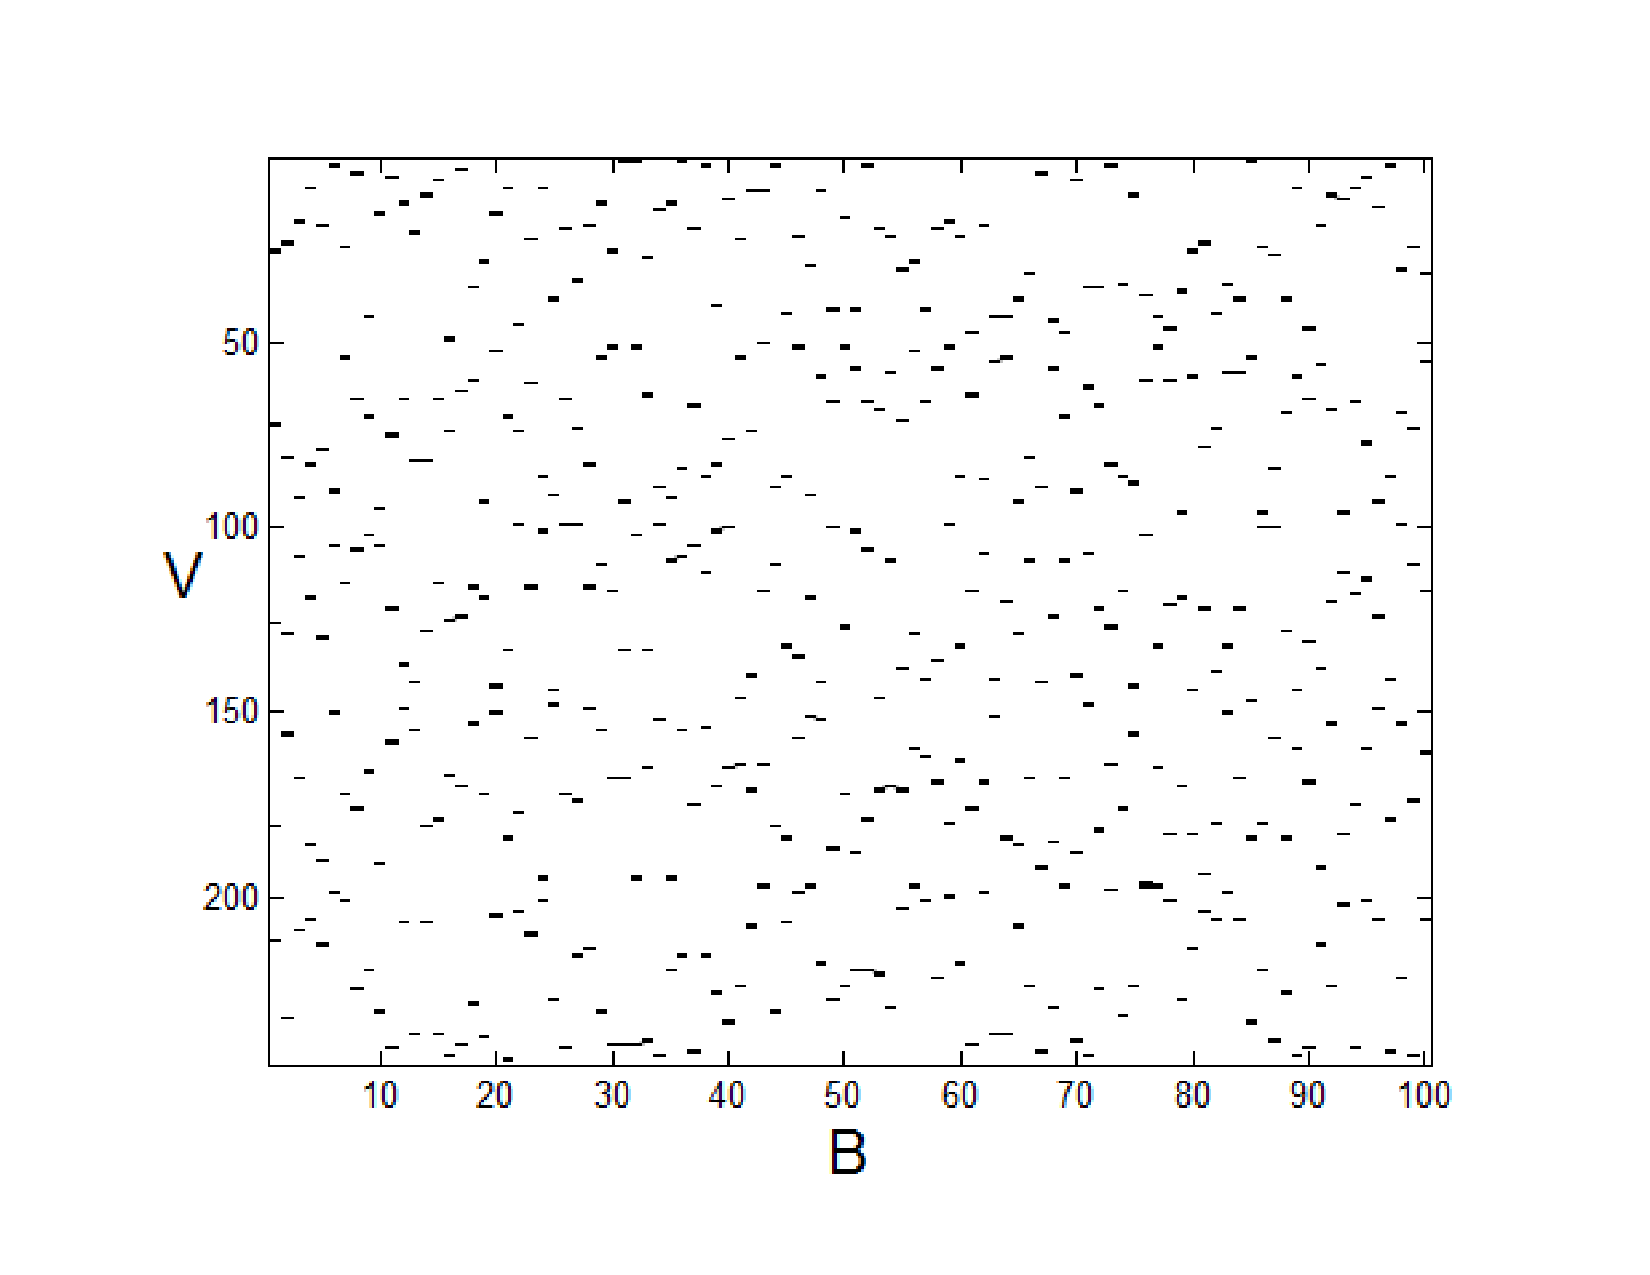
\includegraphics[width=.5\textwidth]{figures/Score(Original).pdf}
\label{fig-6}
}\quad
\subfigure{
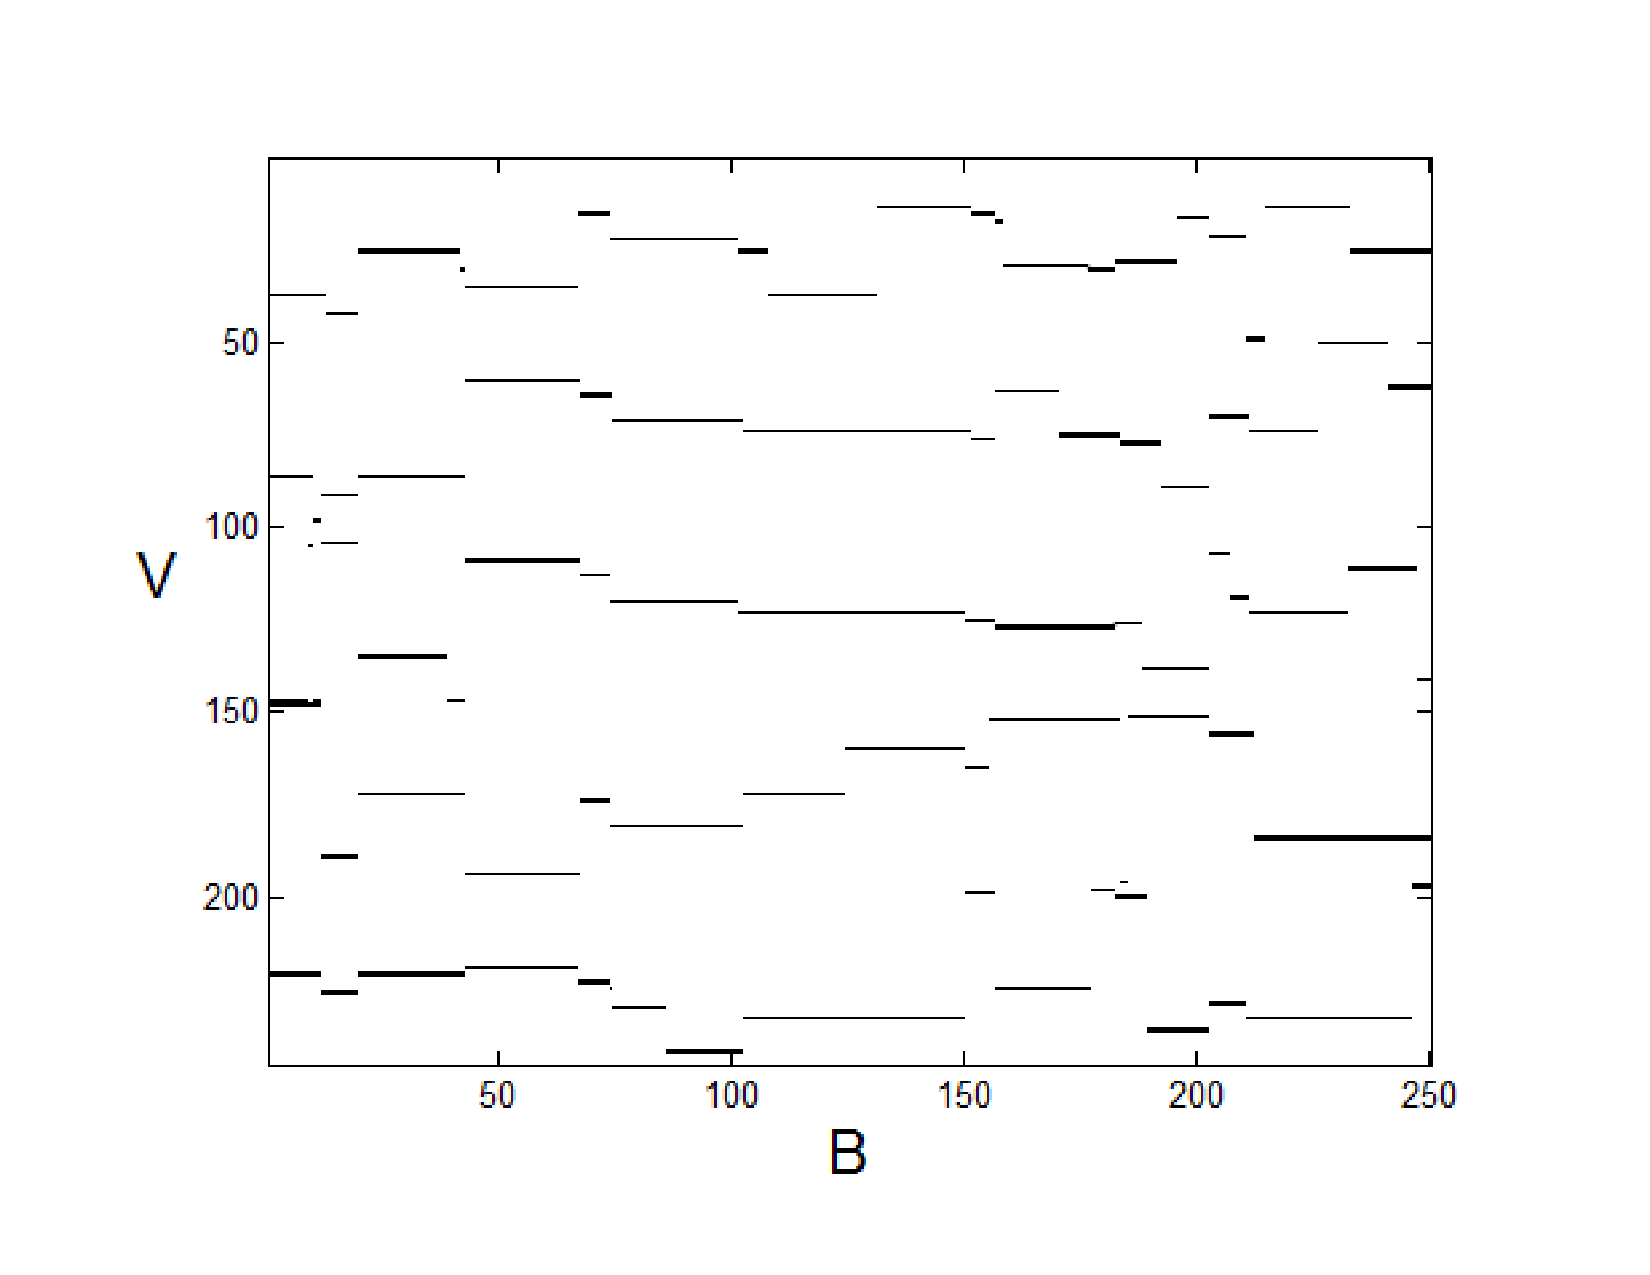
\includegraphics[width=.5\textwidth]{figures/Score(Sampled).pdf}
\label{fig-7}
}
}
\centering
\caption{Comparison of Original and Sampled Scores}
\label{fig-all}
\end{figure}

\end{document}